\begin{singlespace}
    \chapter{\textbf{Appendix B: Supplemental material for "Soil nitrogen availability modifies leaf nitrogen economies in mature temperate deciduous forests: a direct test of photosynthetic least-cost theory"}}
\end{singlespace}

\setcounter{table}{0}
\renewcommand{\thetable}{B\arabic{table}}

\setcounter{figure}{0}
\renewcommand{\thefigure}{B\arabic{figure}}

\begin{table}[h!]
    \caption[Sample sizes of each species, abbreviated by their USDA NRCS PLANTS database code, within each plot at each site]{Sample sizes of each species, abbreviated by their USDA NRCS PLANTS database code, within each plot at each site$^*$}
    \label{table:tab.b1}
    \resizebox{\textwidth}{!}{%
    \begin{tabular}{p{0.5cm}p{2cm}|p{1cm}p{1cm}p{1cm}p{1cm}p{1cm}|p{1cm}}
        \hline
        \multicolumn{2}{l}{} &
        \multicolumn{1}{l}{ACRU} &
        \multicolumn{1}{l}{ACSA} &
        \multicolumn{1}{l}{FAGR} &
        \multicolumn{1}{l}{FRAM} &
        \multicolumn{1}{l}{QURU} &
        \multicolumn{1}{l}{$N_\mathrm{plot}$} \\
        \hline
        \multicolumn{2}{l}{Bald Hill} &
        &&&&&\\
                    & +N; +S                & 0  & 6  & 1  & 0  & 1  & 8  \\
                    & +N; $-$S              & 1  & 2  & 2  & 0  & 1  & 6  \\
                    & $-$N; +S              & 2  & 2  & 0  & 0  & 2  & 6  \\
                    & $-$N; $-$S            & 2  & 3  & 3  & 0  & 2  & 10 \\
        \multicolumn{2}{l}{Carter Creek}    &    &    &    &    &    &    \\
                    & +N; +S                & 0  & 6  & 1  & 2  & 0  & 9  \\
                    & +N; $-$S              & 0  & 4  & 0  & 2  & 0  & 6  \\
                    & $-$N; +S              & 0  & 5  & 1  & 4  & 0  & 10 \\
                    & $-$N; $-$S            & 0  & 7  & 0  & 0  & 0  & 7  \\
        \multicolumn{2}{l}{Mount Pleasant}  &    &    &    &    &    &    \\
                    & +N; +S                & 3  & 2  & 1  & 0  & 3  & 9  \\
                    & +N; $-$S              & 0  & 5  & 4  & 1  & 0  & 10 \\
                    & $-$N; +S              & 1  & 2  & 4  & 0  & 0  & 7  \\
                    & $-$N; $-$S            & 3  & 3  & 1  & 2  & 1  & 10 \\
      \hline
      \multicolumn{2}{l}{$N_\mathrm{spp}$}  & 12 & 47 & 18 & 11 & 10 & 98
      \end{tabular}%
      }
      \end{table}
      \begin{singlespace}
        \noindent $^*$Plots within each site are represented based on nitrogen and sulfur addition status. The final column on the right depicts total sample size per plot in each site ($N_\mathrm{plot}$) and the final row on the bottom represents cumulative species sample size across all plots and all sites ($N_\mathrm{spp}$). Key: ACRU=\textit{A. rubrum}; ACSA=\textit{A. saccharum}; FAGR=\textit{F. grandifolia}; FRAM=\textit{F. americana}; QURU=\textit{Q. rubra}
      \end{singlespace}
    \clearpage

    \newpage
    \begin{table}[]
        \caption[Analysis of variance results exploring the linear effect of leaf temperature on net photosynthesis rate and stomatal conductance measured at 400 $\mu \mathrm{mol\ mol^{-1}\ CO_2}$]{Analysis of variance results exploring the linear effect of leaf temperature on net photosynthesis rate ($A_\mathrm{net}$; $\mathrm{\mu mol\ m^{-2}\ s^{-1}}$) and stomatal conductance ($g_\mathrm{sw}$; $\mathrm{\mu mol\ m^{-2}\ s^{-1}}$) measured at 400 $\mu \mathrm{mol\ mol^{-1}\ CO_2}$}
        \centering
        \label{table:tab.b2}
        %\resizebox{\textwidth}{!}{%
        \begin{tabular}{p{4cm}p{0.5cm}p{3cm}p{3m}p{3cm}p{3cm}}
            && \multicolumn{2}{r}{$A_\mathrm{net}$} & \multicolumn{2}{r}{$g_\mathrm{sw}$} \\
            \hline
            & df                    
            & \multicolumn{1}{r}{$\chi^2$}      & \multicolumn{1}{r}{\textit{p}}
            & \multicolumn{1}{r}{$\chi^2$}      & \multicolumn{1}{r}{\textit{p}}
            \\
            \hline
            
            Leaf temperature & 1    
            & \multicolumn{1}{r}{1.287}         & \multicolumn{1}{r}{0.257}      
            & \multicolumn{1}{r}{1.716}         & \multicolumn{1}{r}{0.190} \\

\end{tabular}%
%}
\end{table}
\begin{singlespace}
\noindent $^*$Results detail linear mixed effects model where temperature was regressed against net photosynthesis or stomatal conductance, with site and species designated as random intercept terms. Significance was determined using Type II Wald $\chi^2$ tests ($\alpha$=0.05).
\end{singlespace}
\clearpage

\newpage
\begin{table}[]
    \centering
    \caption[Second order log-polynomial regression coefficients that described the effect of leaf temperature on net photosynthesis and stomatal conductance measured at 400 $\mu \mathrm{mol\ mol^{-1}\ CO_2}$]{Second order log-polynomial regression coefficients that described the effect of leaf temperature on net photosynthesis ($A_\mathrm{net}$; $\mathrm{\mu mol\ m^{-2}\ s^{-1}}$) and stomatal conductance ($g_\mathrm{sw}$; $\mathrm{\mu mol\ m^{-2}\ s^{-1}}$) measured at 400 $\mu \mathrm{mol\ mol^{-1}\ CO_2}^*$}
    \label{table:tab.b3}
    %\resizebox{\textwidth}{!}
\end{table}
\begin{singlespace}
    \noindent $^*$Net photosynthesis and stomatal conductance values were fit to the log-polynomial equation log(y)= a + bx + cx$^2$, where x is leaf temperature in \textdegree{}C.
\end{singlespace}
\clearpage

\newpage
\begin{landscape}
\begin{table}[]
    \caption[Mean, standard error, and 95\% confidence interval ranges of soil nitrogen availability estimates across all measured plots]{Mean, standard error, and 95\% confidence interval ranges of soil nitrogen availability estimates across all measured plots. All units are expressed as $\mu \mathrm{g\ N\ g^{-1}\ resin\ d^{-1}}$}
    \centering
    \label{tab:table.b4}
    %\resizebox{\columnwidth}{!}{%
    \begin{tabular}{p{3cm}p{3.5cm}p{1.5cm}p{1.5cm}p{2.75cm}p{2.75cm}}
        \hline
        Site           & Treatment        & \multicolumn{1}{r}{Mean }   & \multicolumn{1}{r}{SE}    & \multicolumn{1}{r}{Lower 95\% CI} & \multicolumn{1}{r}{Upper 95\% CI} \\
        \hline
        Bald Hill      & Ammonium sulfate & \multicolumn{1}{r}{27.11}   & \multicolumn{1}{r}{6.14}  & \multicolumn{1}{r}{15.08}         & \multicolumn{1}{r}{39.13}  \\
        Bald Hill      & Control          & \multicolumn{1}{r}{14.41}   & \multicolumn{1}{r}{5.02}  & \multicolumn{1}{r}{4.56}          & \multicolumn{1}{r}{24.26}  \\
        Bald Hill      & Sodium nitrate   & \multicolumn{1}{r}{20.65}   & \multicolumn{1}{r}{3.15}  & \multicolumn{1}{r}{14.46}         & \multicolumn{1}{r}{26.83}  \\
        Bald Hill      & Sulfur           & \multicolumn{1}{r}{6.33}    & \multicolumn{1}{r}{2.19}  & \multicolumn{1}{r}{2.04}          & \multicolumn{1}{r}{10.62}  \\
        Carter Creek   & Ammonium sulfate & \multicolumn{1}{r}{26.94}   & \multicolumn{1}{r}{5.36}  & \multicolumn{1}{r}{16.43}         & \multicolumn{1}{r}{37.44}  \\
        Carter Creek   & Control          & \multicolumn{1}{r}{19.87}   & \multicolumn{1}{r}{1.92}  & \multicolumn{1}{r}{16.10}         & \multicolumn{1}{r}{23.64}  \\
        Carter Creek   & Sodium nitrate   & \multicolumn{1}{r}{15.51}   & \multicolumn{1}{r}{4.16}  & \multicolumn{1}{r}{7.36}          & \multicolumn{1}{r}{23.65}  \\
        Carter Creek   & Sulfur           & \multicolumn{1}{r}{5.50}    & \multicolumn{1}{r}{1.40}  & \multicolumn{1}{r}{2.75}          & \multicolumn{1}{r}{8.25}   \\
        Mount Pleasant & Ammonium sulfate & \multicolumn{1}{r}{8.02}    & \multicolumn{1}{r}{2.31}  & \multicolumn{1}{r}{3.49}          & \multicolumn{1}{r}{12.56}  \\
        Mount Pleasant & Control          & \multicolumn{1}{r}{2.00}    & \multicolumn{1}{r}{0.57}  & \multicolumn{1}{r}{0.89}          & \multicolumn{1}{r}{3.11}   \\
        Mount Pleasant & Sodium nitrate   & \multicolumn{1}{r}{2.52}    & \multicolumn{1}{r}{0.68}  & \multicolumn{1}{r}{1.19}          & \multicolumn{1}{r}{3.85}   \\
        Mount Pleasant & Sulfur           & \multicolumn{1}{r}{2.42}    & \multicolumn{1}{r}{0.39}  & \multicolumn{1}{r}{1.66}          & \multicolumn{1}{r}{3.17} \\
        \hline        
    \end{tabular}%}
    \end{table}
\end{landscape}
\clearpage

\newpage
\begin{landscape}
    \begin{figure}
        \centering
        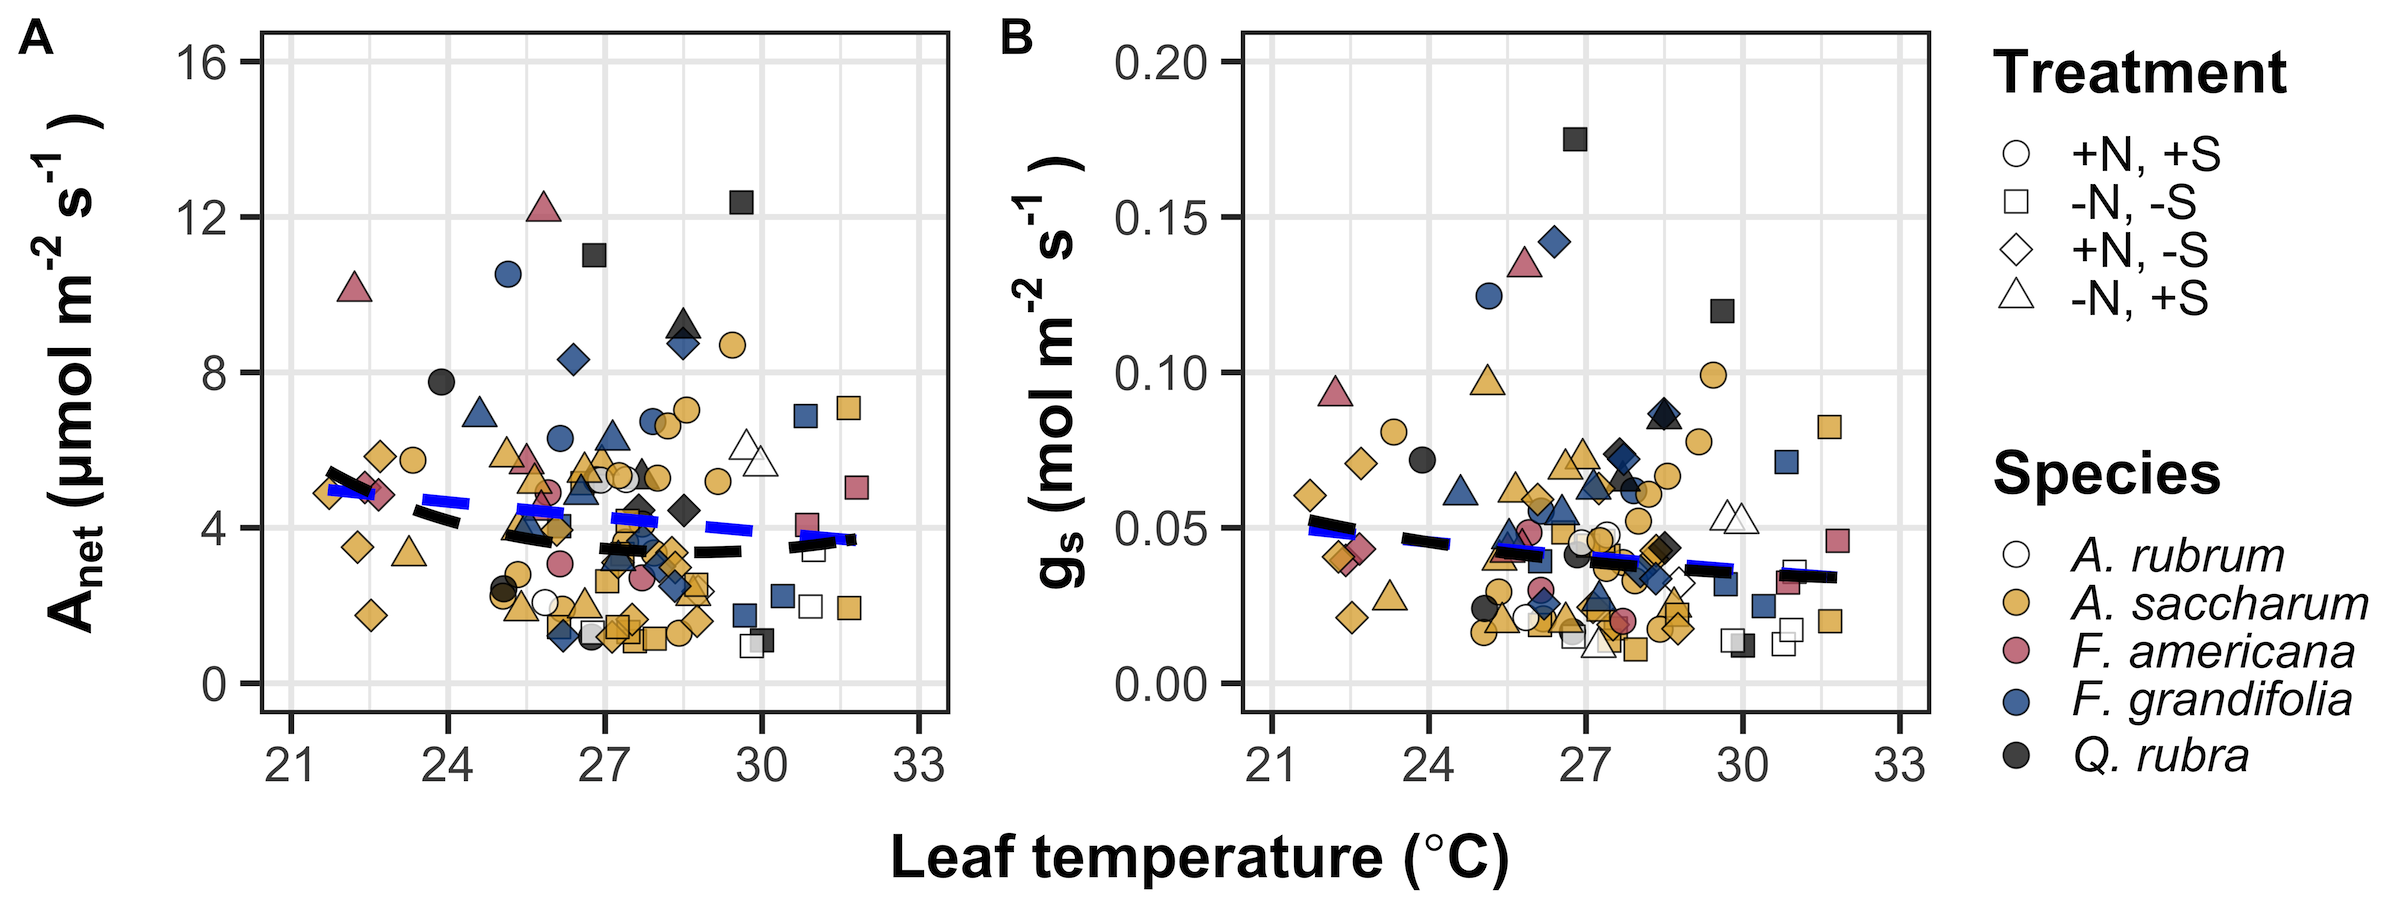
\includegraphics[scale = 0.07]{ch3_NxpH/figs/NxS_figS1_leaftemp.png}
        \caption[Effects of leaf temperature on net photosynthesis rate and stomatal conductance values when measured at 400 $\mu \mathrm{mol\ mol^{-1}\ CO_2}$]{Effects of leaf temperature on net photosynthesis rate (A) and stomatal conductance (B) values when measured at 400 $\mu \mathrm{mol\ mol^{-1}\ CO_2}$. Leaf temperature is represented on the x-axis, while species are represented as colored points. Colored points and shapes are as explained in Figure \ref{fig:figure3.1}. The dashed blue trendline describes the linear relationship between leaf temperature and each response variable, while the dashed black trendline describes the same relationship with a log-polynomial regression equation.}
        \label{fig:figure.b1}
    \end{figure}
\end{landscape}
\clearpage
